
\documentclass[11pts,a4paper,amsmath,amssymb,floatfix]{book}

%\usepackage[gather]{chapterbib}

\usepackage{graphicx,wrapfig}% Include figure files
%\usepackage{dcolumn,enumerate}% Align table columns on decimal point
\usepackage{enumerate}% Align table columns on decimal point
\usepackage{bm,dpfloat}% bold math
\usepackage[pdftex,bookmarks,colorlinks=true,urlcolor=rltblue,citecolor=blue]{hyperref}
\usepackage{amsfonts,amsmath,amsthm,amssymb,stmaryrd,indentfirst}
\usepackage{times,psfrag,pdfpages}
\usepackage[sort&compress,comma,authoryear]{natbib}
\usepackage{color}
\usepackage{units}
\usepackage{rotating}
\usepackage{multirow}

%\usepackage{algorithm}
\usepackage[linesnumbered,lined,boxed,commentsnumbered]{algorithm2e}
%[ruled,vlined][linesnumbered,lined,boxed,commentsnumbered]

\usepackage[noend]{algpseudocode}
\makeatletter
\def\BState{\State\hskip-\ALG@thistlm}
\makeatother

\usepackage{pifont}
\usepackage{subfigure}
\usepackage{subeqnarray}
\usepackage{ifthen}
\usepackage{cancel}

\usepackage{supertabular}
\usepackage{moreverb}
\usepackage{fancyvrb}
\usepackage{listings}
\usepackage{palatino}
%\usepackage{doi}
\usepackage{longtable}
\usepackage{float}
%\usepackage{perpage}
%\MakeSorted{figure}
\usepackage{framed}
\definecolor{shadecolor}{gray}{0.9}
%\usepackage{pdflscape}

% Appendix allows the inclusion of a line for "appendices", which otherwise won't get the right page number. You must
% use the [toc] option.
%\usepackage[toc]{appendix}% Text + Eqn box:

%\usepackage[framemethod=TikZ]{./mdframed/mdframed}
%\usepackage{lipsum}
%\mdfdefinestyle{JFrame}{%
%    linecolor=blue,
%    outerlinewidth=1pt,
%    roundcorner=20pt,
%    innertopmargin=\baselineskip,
%    innerbottommargin=\baselineskip,
%    innerrightmargin=20pt,
%    innerleftmargin=20pt, 
%    backgroundcolor=blue!10!white}

%\usepackage[framemethod=default]{./mdframed/mdframed}
%\usepackage{showexpl}
%\mdfdefinestyle{exampledefault}{%
%rightline=true,innerleftmargin=10,innerrightmargin=10,
%frametitlerule=true,frametitlerulecolor=green,
%frametitlebackgroundcolor=yellow,
%frametitlerulewidth=2pt}

\definecolor{rltblue}{rgb}{0,0,0.75}

%\usepackage{natbib}
\usepackage{fancyhdr} %%%%
\pagestyle{fancy}%%%%
% with this we ensure that the chapter and section
% headings are in lowercase
\renewcommand{\chaptermark}[1]{\markboth{#1}{}}
\renewcommand{\sectionmark}[1]{\markright{\thesection\ #1}}
\fancyhf{} %delete the current section for header and footer
%\fancyhead[LE,RO]{\bfseries\thepage}
%\fancyfoot[LE,RO]{\bfseries\thepage}
\fancyhead[LO]{\bfseries\rightmark}
\fancyhead[RE]{\bfseries\leftmark}
\renewcommand{\headrulewidth}{0.5pt}
% make space for the rule
\fancypagestyle{plain}{%
\fancyhead{} %get rid of the headers on plain pages
\renewcommand{\headrulewidth}{0pt} % and the line
}

\def\newblock{\hskip .11em plus .33em minus .07em}
\usepackage{color}

\theoremstyle{definition}
%\newtheorem{exmp}{Example}[chapter]

\newenvironment{fminipage}%
{\fbox{\begin{minipage}}%
{\end{minipage}}}

% For theorems, lemma, proposition and corollary
\theoremstyle{plain}
\newtheorem{thm}{Theorem}[section]
\newtheorem{lem}[thm]{Lemma}
\newtheorem{prop}[thm]{Proposition}
\newtheorem*{cor}{Corollary}
\theoremstyle{definition}
\newtheorem{defn}{Definition}[section]
\newtheorem{conj}{Conjecture}[section]
\newtheorem{exmp}{Example}[section]
\theoremstyle{remark}
\newtheorem*{rem}{Remark}
\newtheorem*{note}{Note}



%\newtheorem{theorem}{Theorem}[section]
%\newtheorem{corollary}{Corollary}[theorem]
%\newtheorem{lemma}[theorem]{Lemma}

\usepackage{makeidx}
\makeindex

\setlength\textwidth      {16.cm}
\setlength\textheight     {23.0cm}
\setlength\oddsidemargin  {-0.3cm}
\setlength\evensidemargin {0.3cm}

\setlength\headheight{14.49998pt} 
\setlength\topmargin{0.0cm}
\setlength\headsep{1.cm}
\setlength\footskip{-0.5cm}
\setlength\parskip{0pt}
\setlength\parindent{0pt}
%%%
%%% Headers and Footers
%\lhead[\text{\small{WORK IN PROGRESS}}] {\text{\small{ICON/AMCG}}} 
%-\lhead[] {\text{\small{ICON/AMCG}}} 
%-\chead[\text{\small{FETCH Manual}}]  {\text{\small{FETCH Manual}}} %{\text{\small{JAERI Analysis Report Issue}}}
%-\rhead[\text{\small{Commercial-in Confidence}}]{}
\cfoot[\thepage]{\thepage}
%-\rfoot[]{}%{\text{\small{\today}}}
%\cfoot[\text{\small{\today}}]{}% {\text{\small{\today}}}
%\cfoot[\text{\small{January 2006}}] {\text{\small{January 2006}}}
%-\lfoot []{}%{\text{\small{Numerical Analysis}}}
%-\renewcommand{\headrulewidth}{0.8pt}

%%%
%%% space between lines
%%%
\renewcommand{\baselinestretch}{1.5}

\newenvironment{VarDescription}[1]%
  {\begin{list}{}{\renewcommand{\makelabel}[1]{\textbf{##1:}\hfil}%
    \settowidth{\labelwidth}{\textbf{#1:}}%
    \setlength{\leftmargin}{\labelwidth}\addtolength{\leftmargin}{\labelsep}}}%
  {\end{list}}

%%%%%%%%%%%%%%%%%%%%%%%%%%%%%%%%%%%%%%%%%%%
%%%%%%                              %%%%%%%
%%%%%%      NOTATION SECTION        %%%%%%%
%%%%%%                              %%%%%%%
%%%%%%%%%%%%%%%%%%%%%%%%%%%%%%%%%%%%%%%%%%%

% Text abbreviations.
\newcommand{\ie}{{\em{i.e., }}}
\newcommand{\eg}{{\em{e.g., }}}
\newcommand{\cf}{{\em{cf., }}}
\newcommand{\SAA}{{\em{Simulated Annealing Algorithm }}}
\newcommand{\fetch}{FETCH }
\newcommand{\fmips}{FETCH-MIPS }
\newcommand{\bw}{B$\$$W }
\newcommand{\fluidity}{Fluidity }
\newcommand{\event}{{EVENT }}
\newcommand{\gem}{GEM }
\newcommand{\radiant}{RADIANT }
\newcommand{\wrt}{with respect to }
\newcommand{\lhs}{left hand side}
\newcommand{\rhs}{right-hand side }
\newcommand{\vv}{V$\&$V }
\newcommand{\cse}{CS$\&$E }
\newcommand{\amcg}{\href{http://amcg.ese.ic.ac.uk}{AMCG }}
% Commands definining mathematical notation.

% This is for quantities which are physically vectors.
\renewcommand{\vec}[1]{{\mbox{\boldmath$#1$}}}
% Physical rank 2 tensors
\newcommand{\tensor}[1]{\overline{\overline{#1}}}
% This is for vectors formed of the value of a quantity at each node.
\newcommand{\dvec}[1]{\underline{#1}}
% This is for matrices in the discrete system.
\newcommand{\mat}[1]{\mathrm{#1}}


\DeclareMathOperator{\sgn}{sgn}

%\newcommand\qed{\hfill\mbox{$\Box$}}
\newcommand{\re}{{\mathrm{I}\hspace{-0.2em}\mathrm{R}}}
\newcommand{\inner}[2]{\langle#1,#2\rangle}
\renewcommand\leq{\leqslant}
\renewcommand\geq{\geqslant}
\renewcommand\le{\leqslant}
\renewcommand\ge{\geqslant}
\renewcommand\epsilon{\varepsilon}
\newcommand\eps{\varepsilon}
\newcommand{\bmF}{\vec{F}}
\newcommand{\bmphi}{\vec{\phi}}
\newcommand{\bmn}{\vec{n}}
\newcommand{\bmns}{{\textrm{\scriptsize{\boldmath $n$}}}}
\newcommand{\bmi}{\vec{i}}
\newcommand{\bmj}{\vec{j}}
\newcommand{\bmk}{\vec{k}}
\newcommand{\bmx}{\vec{x}}
\newcommand{\bmu}{\vec{u}}
\newcommand{\bmv}{\vec{v}}
\newcommand{\bmr}{\vec{r}}
\newcommand{\bma}{\vec{a}}
\newcommand{\bmg}{\vec{g}}
\newcommand{\bmU}{\vec{U}}
\newcommand{\bmI}{\vec{I}}
\newcommand{\bmq}{\vec{q}}
\newcommand{\bmT}{\vec{T}}
\newcommand{\bmM}{\vec{M}}
\newcommand{\bmtau}{\vec{\tau}}
\newcommand{\bmOmega}{\vec{\Omega}}
\newcommand{\pp}{\partial}
\newcommand{\kaptens}{\tensor{\kappa}}
\newcommand{\tautens}{\tensor{\tau}}
\newcommand{\sigtens}{\tensor{\sigma}}
\newcommand{\etens}{\tensor{\dot\epsilon}}
\newcommand{\ktens}{\tensor{k}}
\newcommand{\half}{{\textstyle \frac{1}{2}}}
\newcommand{\tote}{E}
\newcommand{\inte}{e}
\newcommand{\strt}{\dot\epsilon}
\newcommand{\modu}{|\bmu|}
\newcommand{\summation}{\sum\limits}
% Derivatives
\renewcommand{\d}{\mathrm{d}}
\newcommand{\D}{\mathrm{D}}
\newcommand{\ddx}[2][x]{\frac{\d#2}{\d#1}}
\newcommand{\ddxx}[2][x]{\frac{\d^2#2}{\d#1^2}}
\newcommand{\ddt}[2][t]{\frac{\d#2}{\d#1}}
\newcommand{\ddtt}[2][t]{\frac{\d^2#2}{\d#1^2}}
\newcommand{\ppx}[2][x]{\frac{\partial#2}{\partial#1}}
\newcommand{\ppxx}[2][x]{\frac{\partial^2#2}{\partial#1^2}}
\newcommand{\ppt}[2][t]{\frac{\partial#2}{\partial#1}}
\newcommand{\pptt}[2][t]{\frac{\partial^2#2}{\partial#1^2}}
\newcommand{\DDx}[2][x]{\frac{\D#2}{\D#1}}
\newcommand{\DDxx}[2][x]{\frac{\D^2#2}{\D#1^2}}
\newcommand{\DDt}[2][t]{\frac{\D#2}{\D#1}}
\newcommand{\DDtt}[2][t]{\frac{\D^2#2}{\D#1^2}}
% Norms
\newcommand{\Ltwo}{\ensuremath{L_2} }

% Units
\newcommand{\m}[1][]{\unit[#1]{m}}
\newcommand{\km}[1][]{\unit[#1]{km}}
\newcommand{\s}[1][]{\unit[#1]{s}}
\newcommand{\invs}[1][]{\unit[#1]{s}\ensuremath{^{-1}}}
\newcommand{\ms}[1][]{\unit[#1]{m\ensuremath{\,}s\ensuremath{^{-1}}}}
\newcommand{\mss}[1][]{\unit[#1]{m\ensuremath{\,}s\ensuremath{^{-2}}}}
\newcommand{\K}[1][]{\unit[#1]{K}}
\newcommand{\PSU}[1][]{\unit[#1]{PSU}}
\newcommand{\Pa}[1][]{\unit[#1]{Pa}}
\newcommand{\kg}[1][]{\unit[#1]{kg}}
\newcommand{\rads}[1][]{\unit[#1]{rad\ensuremath{\,}s\ensuremath{^{-1}}}}
\newcommand{\kgmm}[1][]{\unit[#1]{kg\ensuremath{\,}m\ensuremath{^{-2}}}}
\newcommand{\kgmmm}[1][]{\unit[#1]{kg\ensuremath{\,}m\ensuremath{^{-3}}}}
\newcommand{\Nmm}[1][]{\unit[#1]{N\ensuremath{\,}m\ensuremath{^{-2}}}}

% Dimensionless numbers
\newcommand{\dimensionless}[1]{\mathrm{#1}}
\renewcommand{\Re}{\dimensionless{Re}}
\newcommand{\Ro}{\dimensionless{Ro}}
\newcommand{\Fr}{\dimensionless{Fr}}
\newcommand{\Bu}{\dimensionless{Bu}}
\newcommand{\Ri}{\dimensionless{Ri}}
\renewcommand{\Pr}{\dimensionless{Pr}}
\newcommand{\Pe}{\dimensionless{Pe}}
\newcommand{\Ek}{\dimensionless{Ek}}
\newcommand{\Gr}{\dimensionless{Gr}}
\newcommand{\Ra}{\dimensionless{Ra}}
\newcommand{\Sh}{\dimensionless{Sh}}
\newcommand{\Sc}{\dimensionless{Sc}}


% Journals
\newcommand{\IJHMT}{{\it International Journal of Heat and Mass Transfer}}
\newcommand{\NED}{{\it Nuclear Engineering and Design}}
\newcommand{\ICHMT}{{\it International Communications in Heat and Mass Transfer}}
\newcommand{\NET}{{\it Nuclear Engineering and Technology}}
\newcommand{\HT}{{\it Heat Transfer}}   
\newcommand{\IJHT}{{\it International Journal for Heat Transfer}}


\newcommand{\frc}{\displaystyle\frac}
\newcommand{\red}{\textcolor{red}}
\newcommand{\blue}{\textcolor{blue}}
\newcommand{\green}{\textcolor{green}}
\newcommand{\purple}{\textcolor{purple}}
\newcommand{\PN}[2][error]{P$_{#1}$DG-P$_{#2}$}
\newcommand{\PNDG}[2][error]{P$_{#1}$DG-P$_{#2}$DG}
%\newcommand{\PNDG}[3][error]{P$_{#1}$DG-P$_{#2}$DG$_{#3}$}
\newcommand{\Partial}[3][error]{\left(\frc{\partial #1}{\partial #2}\right)_{#3}}
\newcommand{\mfr}[3][error]{#1_{#2}^{\left(#3\right)}}
\newcommand{\PermTensor}[1]{\underline{\underline{#1}}\left(\underline{x}\right)}
\newcommand{\PermComp}[1]{\left[#1\left(x\right)\right]_{ij}}
%{P$_{#1}$DG-P$_{#2}$DG}%$_{#3}$}

%%% TIKz
\usepackage{inputenc}
\usepackage{tikz}
\usetikzlibrary{shapes,arrows}

%%%%%%%%%%%%%%%%%%%%%%%%%%%%%%%%%%%%%%%%%%%
%%%%%%                              %%%%%%%
%%%%%% END OF THE NOTATION SECTION  %%%%%%%
%%%%%%                              %%%%%%%
%%%%%%%%%%%%%%%%%%%%%%%%%%%%%%%%%%%%%%%%%%%

% Cause numbering of subsubsections. 
%\setcounter{secnumdepth}{8}
%\setcounter{tocdepth}{8}

\setcounter{secnumdepth}{4}%
\setcounter{tocdepth}{4}%

\newcounter{qcounter}
\includeonly{Module_01, Module_02}
%\includeonly{model_introduction, model_reservoir_equations, model_description}
\DeclareMathAlphabet{\mathpzc}{OT1}{pzc}{m}{it}

%%
%% Short Abstract at the beginning of each chapter
%%
%%%% Option 1:
\usepackage{changepage}
%%%% Option 2:
%\newenvironment{chapabstract}{%
%    \begin{center}%
%      %\bfseries Chapter Abstract
%      \bfseries 
%    \end{center}}%





\begin{document}

\vspace{4cm}

\begin{titlepage}
  \begin{center}
   %  
\includegraphics[width=15cm,clip]{./FigBanner/UoAHorizBanner}
\vspace{3.5cm}

       {\bf{\Huge Integrated Multi-Fluid Flows and Stochastic Upscaling Models}}

\bigskip
       {\bf{\huge Model Documentation}}

\vspace{3.5cm}

  \end{center}

  \begin{tabular}{l c l}
     {\bf{\large Authors:}}                         &     & B. Lashore, J.L.M.A. Gomes \\
                                                    &     & Fluid and Structures Group \\
                                                    &     & School of Engineering \\
                                                    &     & University of Aberdeen \\
\bigskip
     {\bf{\large Date:}}                            &     &   \today                    \\
                                                    &     &                             \\
     {\bf{\large Revision 1:}}                      &     &  April 11, 2017  \\
     {\bf{\large Revision 2:}}                      &     &  \today                     \\
                                                    &     &                             \\
  \end{tabular}
\vspace{3.5cm}

\bigskip

\bigskip


   
\includegraphics[width=15cm,clip]{./FigBanner/UoAHorizBanner}



\end{titlepage}

\setcounter{page}{1}

\tableofcontents
\vfill

%\pagebreak
%\listoftables
%\vfill
%\pagebreak
%\listoffigures
%\vfill
%\pagebreak

%%%
%%% CHAPTER
%%%
\chapter{Multi-Fluids Porous Media Flow Model}\label{ChapterMultiFluidsModel}

%%% Summary of the Chapter
\begin{adjustwidth}{1cm}{1cm}
   {\it The main aim of this chapter is to describe the multiphase porous media flow model used throughout this documentation. This chapter introduces the novel CVFEM formulation with new element-pairs that ensure high-order numerical accuracy in time and space of the set of conservative equations. In summary, pressure and velocities of all phases/fluids are discretised and solved in finite element space whereas scalar fields (\eg saturation, density, temperature etc) are solved in control volume space. Finite element pressure and velocity fields are projected in CV space in order to obtain high-order fluxes on the control volume boundaries. 
\medskip

The contents of this chapter were taken from \citet{gomes_2016} and \citet{Fluidity_Manual}.}
\end{adjustwidth}

%%% SECTION
\section{Numerical Formulation: Force Balance Model}\label{ChapterMultiFluidsModel:Section:overlapping_method_section}

\subsection{A novel representation of multi-phase Darcy flows}\label{ChapterMultiFluidsModel:Section:DarcyModel}
Darcy's law for immiscible multi-phase flow may be written in the form:
\begin{equation}\label{e:darcy_eqn}
  \mathbf{q}_{\alpha} = -\frac{\mathcal{K}_{{r}_\alpha}\mathbf{K}}{\mu_{\alpha}}\left(\nabla p_{\alpha} - {\mathbf{s}_{u}}_{\alpha} \right),
\end{equation}
where $\mathbf{q}_{\alpha}$ is the $\alpha$-th phase Darcy velocity, $\mathbf{K}$ is the absolute permeability tensor of the porous medium, $\mathcal{K}_{{r}_\alpha}\left(S_{\alpha}\right)$ is the phase relative permeability, which is a function of the phase saturation $S_{\alpha}\left(\mathbf{r},t\right)$. $\mu_{\alpha}$, $p_{\alpha}$, $\rho_{\alpha}$, and $\mathbf{s}_{{u}_\alpha}$ are the phase dynamic viscosity, pressure, density and source term, which may include gravity and/or capillarity, respectively. 

Introducing a saturation-weighted Darcy velocity defined as $\mathbf{u}_\alpha= \mathbf{q}_\alpha/S_\alpha$, then Eqn.~\ref{e:darcy_eqn} may be rewritten as:
\begin{equation}
  \mathbf{v}_\alpha={\underline {\underline \sigma}}_{\alpha} \mathbf{u}_{\alpha} = - \nabla p_{\alpha} + {\mathbf{s}_{u}}_{\alpha},
  \label{force-bal}
\end{equation}
where ${\underline {\underline \sigma}}_{\alpha}=\mu_\alpha S_\alpha \left(\mathcal{K}_{{r}_\alpha}\mathbf{K}\right)^{-1}$ represents the implicit linearisation of the viscous frictional forces. The force per unit volume $\mathbf{v}_\alpha$, defined as ${\underline {\underline \sigma}}_{\alpha} \mathbf{u}_\alpha$, is used as a prognostic variable in this approach, as explained in Section~\ref{ChapterMultiFluidsModel:Section:Force_density}.

In order to discretise Eqn.~\ref{force-bal}, a finite element representation for $\mathbf{v}_\alpha$ and $p$ is assumed, expressed in terms of their FE basis functions $Q_{j}$ and $P_{j}$, respectively, as:
\begin{equation}
  \mathbf{v}_\alpha(\bm{r},t) = \sum\limits_{j=1}^{\mathcal{N}_u} Q_{j}(\bm{r})\mathbf{v}_{\alpha,j}(t) \;\;\;\;\text{ and } \;\;\;\; p(\bm{r},t) = \sum\limits_{j=1}^{\mathcal{N}_p} P_{j}(\bm{r})p_{j}(t).
\end{equation} 
Here $\mathcal{N}_{u}$ and $\mathcal{N}_{p}$ are the total number of degrees of freedom for the FE force and pressure representations. Each component of the weak form of the force balance (Eqn.~\ref{force-bal}) is tested with the $\mathbf{v}_\alpha$ basis function space to obtain:
\begin{displaymath}
  \sum\limits_{E} \left. \int\limits_{\Omega_E} { {Q}}_i \left({\mathbf v}_\alpha + \nabla p  -{\mathbf s}_{u_\alpha}\right) \d V \right. + \displaystyle \oint_{\Gamma_{E}} {Q}_i {\mathbf n} \left(p - \tilde{p}\right) \d\Gamma + \oint_{\Gamma_{\Omega}} {Q}_i {\mathbf n} \left(p - p_\text{bc}\right) \d\Gamma = \bm{0},\nonumber \label{force-semi-disc} 
\end{displaymath} 
where $\Omega_E$ and $\Gamma_{E}$ are the volume and boundary of element $E$, respectively, and $\Gamma_{\Omega}$ is the boundary of the computational domain. The numerical pressure $\tilde{p}$ appearing in the jump condition (second term in Eqn.~\ref{force-semi-disc}) is the arithmetic mean of the potentially discontinuous pressure across the element $E$. This term vanishes when a continuous formulation is used to discretise the pressure field. The last term in Eqn.~\ref{force-semi-disc} is used to weakly enforce the pressure level to $p_\text{bc}$ on a computational domain boundary.

In matrix form, Eqn.~\ref{force-semi-disc} is: 
\begin{equation}
  {\mathbf M} \underline {\mathbf v} = -{\mathbf C} \underline{\mathbf p} + \underline {\mathbf s}_{u}, \label{force-balance-matrix-form}
\end{equation}
where $\underline{\bf v}$ and $\underline{\bf p}$ solution-vectors are defined as:
\begin{eqnarray}
    &&\underline{{\bf v}} = \left( \left( {v_x},{v_y},{v_z} \right)_{1,1}, \left( {v_x},{v_y},{v_z} \right)  _{2,1},\ldots, \left( {v_x},{v_y},{v_z} \right)_{\mathcal{N}_\alpha,\mathcal{N}_u} \right)^{T} \;\text{and} \nonumber \\ 
    && \underline{{\bf p}} = \left(p_1, p_2, p_3, \cdots, p_{\mathcal{N}_p}\right)^T. \nonumber% \nonumber
\end{eqnarray}
$\mathcal{N}_{\alpha}$ is the number of phases and $v_x$, $v_y$ and $v_z$ are the components associated with the $x$, $y$ and $z$ dimensions, respectively. Finally, the mass matrix ${\mathbf M}$, gradient matrix ${\mathbf C}$ and source vector $\underline {\mathbf s}_{u}$ are defined as:
\begin{eqnarray}
     && \left[{\mathbf M}^{(i,j)}\right]_{k,l} = \int_{\Omega} Q_{k} \left[\underline{\underline{\sigma}}_{\alpha}\right]_{i,j} {Q}_{l} \d V, \nonumber \\ 
     && {\left[\bm{C}^{(i,i)}\right]_{k,l} = \int_{\Omega} Q_{k} \frac{\partial P_{l}}{\partial r_i} \d V - \oint_{\Gamma_{E}} \displaystyle\frac{1}{2} Q_{k} n_i^{(E,l)} P_{l} d\Gamma - \oint_{\Gamma_{\Omega}} \displaystyle Q_{k} n_i P_{l} \d\Gamma}, \nonumber \\ 
     && {\left[\bm{s}_{u}^{(i,i)}\right]_{k} = \int_{\Omega} Q_k}\left[{\mathbf s}_{u_\alpha} \right]_i \d V - \oint_{\Gamma_{\Omega}}\displaystyle Q_{k} n_i p_\text{bc} \d\Gamma, \nonumber
\end{eqnarray}
where $i$ and $j$ are dimensions and $k$ and $l$ are the degrees of freedom of element $E$. Here, $\bm{n} = \left(n_{1}, n_{2}, n_{3}\right)^{T}$ is the outward-pointing normal vector of the domain $\Omega$. $\bm{n}^{(E,l)}$ is the normal to the boundary of element $E$ and is outward-pointing if $P_{l}$ takes support on $E$, and inward-pointing otherwise.

\medskip

The saturations are computed in CV space, whereas the permeability tensor $\left(\mathbf{K}\right)$ is assumed piece-wise constant in FE space. Thus the viscous-friction damping tensor $ {\underline {\underline \sigma}}_{\alpha}$ is piece-wise constant within the sub-control volumes defined through intersections between the elements and control volumes (see Fig.~\ref{fem_cv_represent_a}).



\subsection{Control Volume Finite Element types}\label{ChapterMultiFluidsModel:Section:Element_Types}
In the formulation presented here, pressure, velocity, permeability and porosity are represented FE-wise, however saturation, relative permeability and fluid properties such as viscosity and density are represented CV-wise. Figure~\ref{fem_cv_represent_a} displays the two families of element types presented in this paper: Fig.~\ref{fem_cv_represent_a} (a) shows the P$_{n}$DG-P$_{n+1}$ element type, with $n = 1$, in two dimensions (2D). Here, the velocity field is linear and discontinuous (between elements) whilst pressure has a quadratic and continuous (between elements) representation with the CV's span various elements. Figure~\ref{fem_cv_represent_a} (b) shows the P$_{n+1}$DG-P$_{n}$DG element type, with $n = 1$ (also in 2D). Here, the velocity field is quadratic and discontinuous (between elements) whereas pressure has a linear and discontinuous (between elements) representation and the CV's do not span elements.
\begin{figure}[h]
   \vbox{
       \hbox{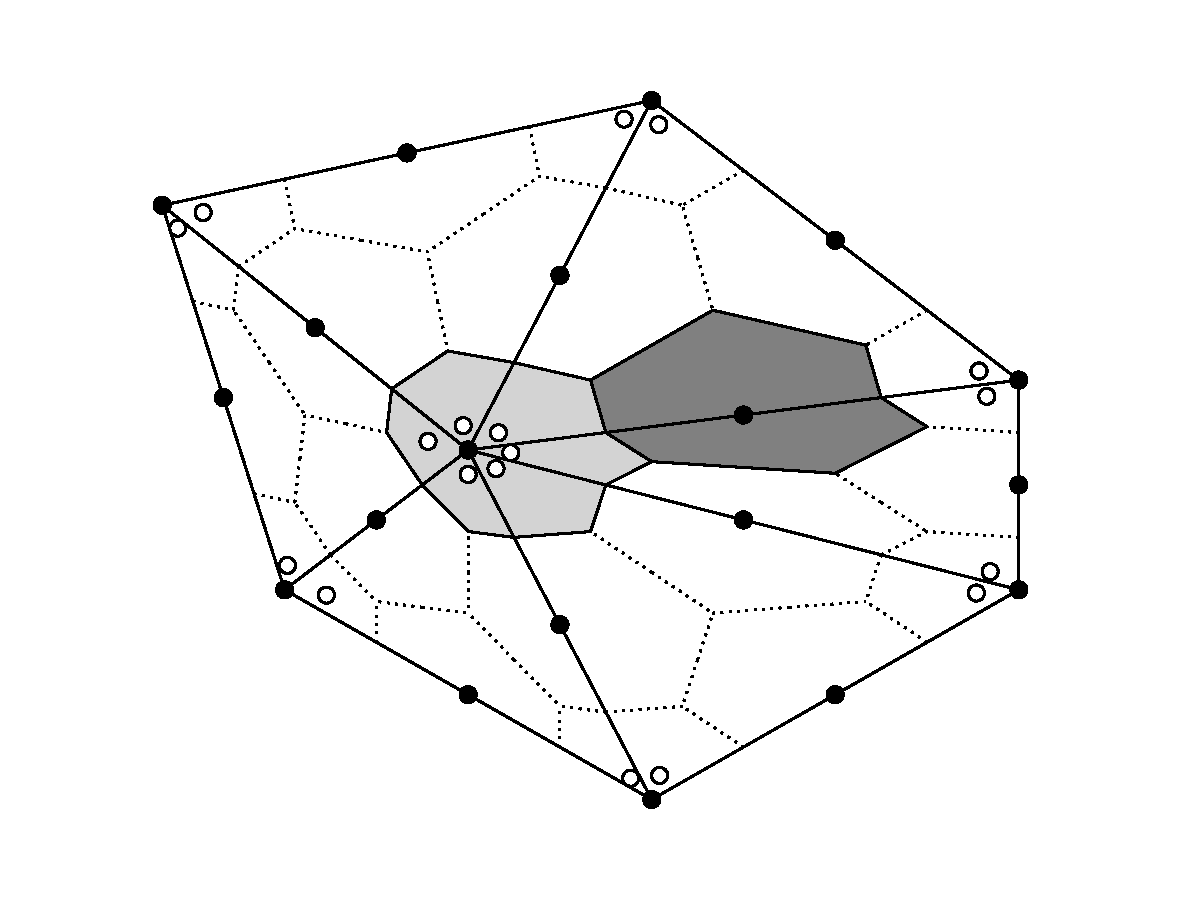
\includegraphics[width=.5\textwidth]{./Figs/p1dgp2-cont-sat.pdf}
             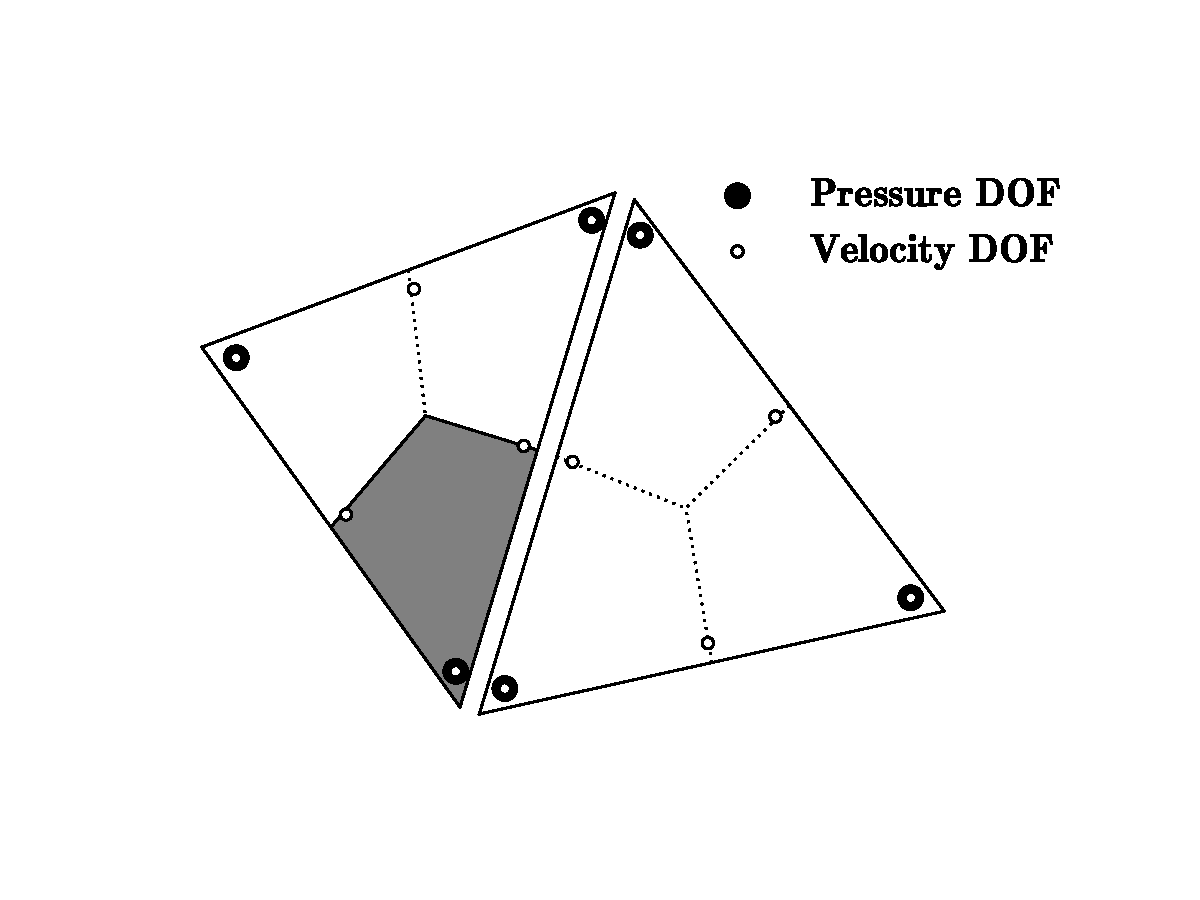
\includegraphics[width=.5\textwidth]{./Figs/p2dgp1-dg-sat.pdf}}
       \hbox{\hspace{3cm}(a) \PN[1]{2} \hspace{5.cm} (b)\PNDG[2]{1}}}
\caption{2D representation of the element pairs presented in this work. Shaded areas denote control volumes (in which saturation is   stored), black points represent the pressure nodes and white points the velocity nodes. Note that in (b) velocity and pressure nodes overlap in the triangles' vertices.}
    \label{fem_cv_represent_a}
\end{figure} 

\subsection{Finite element representation of velocity}\label{ChapterMultiFluidsModel:Section:Force_density}
From Eqn.~\ref{e:darcy_eqn}, it can be seen that the velocity field depends, among other fields, on the absolute permeability which is FE-wise, and the relative permeability which is CV-wise. This means that the velocity representation is different in each CV. However, the quantity $\mathbf{v}_\alpha$ is homogeneous within an element and this is stored using FE representation. To obtain the velocity $\mathbf{u}_{\alpha}$ in a particular CV within a FE, Eqn.~\ref{force-bal} is used.


\section{Saturation and Global Mass Conservative Equations} \label{ChapterMultiFluidsModel:Section:Saturation_Global}
Here, the saturation conservation equations are discretised and the global mass balance equation is derived. In this work, fluids are assumed incompressible. The saturation equation can be written as:
\begin{equation}
  \phi\displaystyle\frac{\partial S_{\alpha} }{\partial t} + \nabla \cdot \left( {\mathbf u}_{\alpha} S_{\alpha}\right) = s_{cty,\alpha}, \label{saturation_equation}
\end{equation}
where $\phi$ is the porosity and $s_{cty}$ is a source term. Eqn.~\ref{saturation_equation} is discretised in space by testing with CV basis functions $M_{i}$ and with the $\theta$-method in time \citep[see][]{gomes_book_2012}:
\begin{eqnarray}
     \int_{\Omega} M_{i} \displaystyle\frac{\phi \left({S_{\alpha i}^{n+1}}-{S_{\alpha i}^{n}}\right)}{\Delta t} \d V + \nonumber  \\ 
     \oint_{\Gamma_{CV_{i}}} \left[\theta^{n+\frac{1}{2}} {\mathbf n}  \cdot {\mathbf u}_{\alpha}^{n+1} S_{\alpha}^{n+1} + \left(1-\theta^{n+\frac{1}{2}}\right) {\mathbf n} \cdot {\mathbf u}_{\alpha}^{n} S_{\alpha}^{n} \right]d\Gamma = \int_{\Omega}  M_{i} {s_{cty,\alpha}^{n+\theta}} \d V, \label{detail-sat-eqn-k}
\end{eqnarray}
where $\mathbf{n}$ is the outward-pointing unit normal vector to the surface ($\Gamma_{CV_{i}}$) of the control volume $i$ and $n$ is the current time level. More details on the numerical methods used to solve Eqn.~\ref{detail-sat-eqn-k} can be found in \citet{pavlidis_2016}.

The global continuity equation is obtained by summing Eqn.~\ref{detail-sat-eqn-k} over all phases:
\begin{eqnarray}
     \sum\limits_{\alpha=1}^{\mathcal{N}_{\alpha}} \left\lbrace \int_{\Omega} M_{i} \displaystyle\frac{\phi\left({S_{\alpha i}^{n+1}}-{S_{\alpha i}^{n}}\right) } {\Delta t} \d V + \right. \nonumber \\ 
     \left. \displaystyle\oint_{{\Gamma_{CV}}_{i}} \left[\theta^{n+\frac{1}{2}} {\mathbf n} \cdot {\mathbf u}_{\alpha}^{n+1} S_{\alpha}^{n+1} + \left(1-\theta^{n+\frac{1}{2}}\right) {\mathbf n} \cdot {\mathbf u}_{\alpha}^{n} S_{\alpha}^{n} \right] \,\d\Gamma - \right. \nonumber \\ 
     \left. \displaystyle\int_{\Omega} M_{i} s_{cty,\alpha}^{n+\theta}\, \d V \right\rbrace = 0. \label{detail-sat-eqn-k-sum}
\end{eqnarray}
Equation~\ref{detail-sat-eqn-k-sum} is also bounded by the constraint:
\begin{equation}
  \sum\limits_{\alpha=1}^{\mathcal{N}_{\alpha}} {S_{\alpha}^{n}}_{i} = 1, \quad \forall n.
\end{equation}
Solving for ${\mathbf u}^{n+1}$ in matrix form, Eqn.~\ref{detail-sat-eqn-k-sum} becomes:
\begin{equation}
  {\mathbf B}^T \underline{\bf v}^{n+1} = \underline{\bf s}_{p}.   \label{glob-cty-matrix}
\end{equation}


\section{Velocity at Control Volume Interfaces} \label{ChapterMultiFluidsModel:Section:opt-up} 
The velocity to be used at the interface between CV's in the saturation conservation (Eqn.~\ref{detail-sat-eqn-k}) and global continuity (Eqn.~\ref{detail-sat-eqn-k-sum}) equations needs to be determined. On the CV faces, there is no information about the flow direction as the velocity is discontinuous at the CV boundaries. The discontinuities occur between (a) control volumes within each FE and (b) between elements when using the \PNDG[n+1]{n} element pair.

In order to calculate the velocity across CV's within a FE, an average velocity at the interface of control volumes {\it i} and {\it j} is defined as:
\begin{equation}
  {\tilde{\bf u}}_\alpha = \frac{1}{2} \left[ {{\bf u}_\alpha}_i + {{\bf u}_\alpha}_j \right].
\end{equation} 
From this, the interface velocities at either side of the interface can be obtained from:
%\begin{equation}
%  {\tilde{\bf u}}_{\alpha k} = \underline{\underline{\sigma}}_{\alpha
%    k}^{-1}{\tilde{{\bf u}}}_{\alpha}, \;\;\;\; k=\{i,j\}.
%  \label{two-vels}
%\end{equation} 
\begin{equation}
  {\tilde{\bf u}}_{\alpha k} = \underline{\underline{\sigma}}_{\alpha k}^{-1}{{\bf \tilde{v}}}_{\alpha}, \;\;\;\; k=\{i,j\}. 
  \label{two-vels}
\end{equation} 

These velocities have the same direction and differ only in magnitude, so using them to define an upwind direction is not ambiguous. If an upwind method for calculating the interface velocity is applied then,
\begin{equation}
  {\tilde{\bf u}}_{\alpha} = \tilde{\bf u}_{\alpha k},\label{interface_velocity_upwind}
\end{equation}
where $k=i$ if ${\bf n}\cdot{\bf u}_{\alpha}>0$ (CV {\it i} outgoing information), and $k=j$ if ${\bf n}\cdot{\bf u}_{\alpha}<0$ (CV {\it i} incoming information). 

However, upwind methods yield dissipative solutions therefore, in order to obtain a high-order approximation of the velocity at the interface, the saturation at the interface $\tilde{S}_{\alpha}$ is calculated using a finite element representation of the saturation following the upwind direction. $\tilde \sigma_{\alpha}$ can then be calculated using second-order Taylor series:
%\begin{small}
\begin{equation}
    \underline{\underline{\tilde{\sigma}}}_{\alpha} = \underline{\underline{\sigma}}_{\alpha k} + \left(\tilde{S}_{\alpha}-S_{\alpha k}\right) \left(\frc{\partial \underline{\underline{\sigma}}_{\alpha}}{\partial S_{\alpha}}\right)_{k} + \frc{1}{2}\left(\tilde{S}_{\alpha}-S_{\alpha k}\right)^{2} \left[ \frc{ \left(\frc{\partial \underline{\underline{\sigma}}_{\alpha}}{\partial S_{\alpha}}\right)_{k} - \left(\frc{\partial \underline{\underline{\sigma}}_{\alpha}}{\partial S_{\alpha}}\right)_{l} } { \left(S_{\alpha k}-S_{\alpha l}\right) } \right], \label{sigma-out}
\end{equation}
%\end{small}
where $k=i$ and $l=j$ if ${\bf n}\cdot{\bf u}_{\alpha}>0$ and, $k=j$ and $l=i$ if ${\bf n}\cdot{\bf u}_{\alpha}<0$. Therefore, the final interface velocity (Eqn.~\ref{interface_velocity_upwind}) can be obtained from:
%\begin{equation}
%  {\tilde{\bf u}_{\alpha}} = \underline{\underline{\tilde{\sigma}}}_{\alpha}^{-1} \left[\displaystyle\frac{1}{2} \left( {{\bf u}_\alpha}_i + {{\bf u}_\alpha}_j \right)\right], \label{mean_int_vel}  
%\end{equation} 
\begin{equation}
  {\tilde{\bf u}_{\alpha}} = \underline{\underline{\tilde{\sigma}}}_{\alpha}^{-1} \left[\displaystyle\frac{1}{2} \left( {{\bf v}_\alpha}_i + {{\bf v}_\alpha}_j \right)\right], \label{mean_int_vel}  
\end{equation} 
%The interface velocity obtained from Eqn.~\ref{mean_int_vel} is bounded to ensure that its normal component ${\tilde{\bf u}_\alpha}\cdot {\bf n}$ lies between ${\tilde{\bf u}_{\alpha i}}\cdot {\bf n}$ and ${\tilde{\bf u}_{\alpha j}}\cdot {\bf n}$. The result of this is also bounded between the velocities ${{\bf u}_\alpha}_i\cdot {\bf n}$ and ${{\bf u}_\alpha}_j\cdot {\bf n}$.
The interface velocity obtained from Eqn.~\ref{mean_int_vel} is bounded to ensure that its normal component ${\tilde{\bf u}_\alpha}\cdot {\bf n}$ lies between ${\tilde{\bf u}_{\alpha i}}\cdot {\bf n}$ and ${\tilde{\bf u}_{\alpha j}}\cdot {\bf n}$. The result of this is also bounded between the velocities ${{\bf v}_\alpha}_i\cdot {\bf n}$ and ${{\bf v}_\alpha}_j\cdot {\bf n}$.

\medskip

In a fully discontinuous formulation with \PNDG[n+1]{n} element pairs, the interface velocity (now between neighbour elements) can not be calculated using Eqn.~\ref{mean_int_vel} due the elliptic nature of the discretised non-symmetric pressure equation, Eqn.~\ref{force-balance-matrix-form}. This means that information is propagated in all directions across the (discontinuous) domain and hence, taking the upwind velocity as commonly done within an element is not an adequate strategy.
 
For two neighbouring CV's $i$ and $j$ with common FE interface ({\it e.g.}, see Fig.~\ref{fem_cv_represent_a}b for \PNDG[2]{1} element pair), $\tilde{\bf u}_\alpha$ can be calculated by using a volume-weighted harmonic mean. However, the volume $\mathcal{V}$ of the control volume and $\underline{\underline{\sigma}}_{\alpha}$ act on the velocity in a very similar way. Hence, the velocity at the interface is expressed as,
\begin{equation} 
  {\tilde{\bf u}_\alpha} =  \left(\mathcal{V}_{j} \underline{\underline{\sigma}}_{\alpha j} \, {\bf u}_{\alpha i} + \mathcal{V}_{i} \underline{\underline{\sigma}}_{\alpha i}\, {\bf u}_{\alpha j} \right) \left(  \mathcal{V}_{i} \underline{\underline{\sigma}}_{\alpha i} + \mathcal{V}_{j}  \underline{\underline{\sigma}}_{\alpha j} \right)^{-1}.
\end{equation} 


\section{Weak Enforcement of Boundary Conditions}\label{ChapterMultiFluidsModel:Section:bcs-rel-perm} 
Suitable boundary conditions for velocity can be applied by the discontinuous formulation above as well as by the upwinding in the continuous formulation. In fact, exactly the same boundary condition implementations, as used in the discontinuous formulation, can be applied across the boundaries of the domain by taking information from `just outside' the domain rather than from the neighbouring elements.

Saturation boundary conditions are relatively straightforward. One typically takes the saturation from `just outside' the domain ($S_{\alpha, \text{bc}}$) and the flux becomes $\left({\bf n}\cdot {\bf u}_{\alpha}\right)S_{\alpha,\text{bc}}$, if ${\bf n}\cdot {\bf u}_{\alpha} < 0$. If the velocity is also specified (${\bf u}_{\alpha,\text{bc}}$) then this becomes part of the incoming flux $\left({\bf n}\cdot {\bf u}_{\alpha,\text{bc}}\right)S_{\alpha,\text{bc}}$.

In case of specified pressure for outflow boundaries $\left(\right.{\bf n}\cdot {\bf u}_\alpha>0\left.\right)$ the flux is ${\bf n}\cdot {\bf u}_\alpha {S_\alpha}$, in which neither ${\bf u}_\alpha$ nor ${S_\alpha}$ are specified. 

However, for inflow boundaries with specified pressure $\left(\right.{\bf n}\cdot {\bf u}_\alpha<0\left.\right)$ the flux is ${\bf n}\cdot {\bf u}_{\alpha,\text{bc}} S_{\alpha,\text{bc}}$, in which ${\bf u}_{\alpha,\text{bc}}$ is calculated using:
\begin{equation}
  {\bf u}_{\alpha,\text{bc}} =  \underline{\underline{\sigma}}_{\alpha,\text{bc}} ^{-1}  \underline{\underline{\sigma}}_{\alpha} {\bf u}_{\alpha},
\end{equation}
where $\underline{\underline{\sigma}}_{\alpha,\text{bc}}$ is calculated using $S_{\alpha,\text{bc}}$. Ut should be noted that this flux condition must be used in both the discretised saturation and global continuity equations, since the latter is a summation of the former. The specified pressure condition becomes a surface flux condition in the force balance equation (Eqn.~\ref{force-semi-disc}), which effectively relaxes the pressure $p$ to its face value counterpart $p_\text{bc}$ at the boundaries.


\section{Solving the linear equations}\label{ChapterMultiFluidsModel:Section:SolvingLinearEqns}
The global mass balance equation (Eqn.~\ref{glob-cty-matrix}) and force balance equations (Eqn.~\ref{force-balance-matrix-form}) are solved by substituting $\underline{\mathbf v}$ and solving the system of equations for pressure. At time level $n+1$, Eqns.~\ref{force-balance-matrix-form} and ~\ref{glob-cty-matrix} can be rewritten as:
\begin{displaymath}
  \begin{cases}
      \mathbf{M} \underline{\bf v}^{n+1} = \mathbf{C}\underline{\bf p}^{n+1} + \underline{\bf s}_{u}^{n+1} \\ 
      \mathbf{B}^{T} \underline{\bf v}^{n+1} = \underline{\bf s}_{p}^{n+1},
  \end{cases}
\end{displaymath}
respectively. Application of a discontinuous FEM for $\mathbf{v}$ leads to a block-diagonal $\mathbf{M}$ matrix that can be readily inverted, each block being local to an element. Multiplying Eqn.~\ref{force-balance-matrix-form} by $\mathbf{B}^{T}\mathbf{M}^{-1}$ and summing up with Eqn.~\ref{glob-cty-matrix}, $\underline{\mathbf v}^{n+1}$ vanishes and the pressure equation is obtained:
\begin{equation}
    \mathbf{B}^{T}\mathbf{M}^{-1} \mathbf{C} \underline{\bf p}^{n+1} =  \underline{\bf s}_{p}^{n+1} - \mathbf{B}^{T} \mathbf{M}^{-1}  \underline{\bf s}_{u}^{n+1}. \label{final_projection}
\end{equation}
Equation~\ref{final_projection} is solved for pressure and then the velocity is obtained via Eqn.~\ref{force-balance-matrix-form}. The computationally demanding effort to solve the pressure matrix equation arising from the fully discontinuous FEM formulation is achieved using a multigrid-like approach \citep[see][]{Brandt}. In this case the `fine' mesh is the one obtained by the discontinuous system, whereas the `coarse' mesh is obtained by creating a continuous system (from the discontinuous system) by collapsing the pressure nodes. As in multigrid, the coarse mesh solution is used to accelerate the convergence of the fine mesh solution by calculating the error of the current approximation.


%%%
%%% CHAPTER
%%%
\chapter{Upscaling Models}\label{Chapter:UpscalingModels}

%%% Summary of the Chapter
\begin{adjustwidth}{1cm}{1cm}
   {\it The main aim of this chapter is to describe the variety of determininstic and stochastic upscaling models and ...}
\medskip
\end{adjustwidth}


%%%
%%% CHAPTER
%%%
\chapter{Upscaling Formulation Model}\label{Chapter:UpscalingFormulationModel}

%%% Summary of the Chapter
\begin{adjustwidth}{1cm}{1cm}
   {\it The main aim of this chapter is to describe the variety of determininstic and stochastic upscaling models and ...}
\medskip
\end{adjustwidth}


\section{Definitions}\label{Chapter:UpscalingFormulationModel:Section:Definitions}

Given an open bounded domain $\Omega\subset\mathbb{R}^{d}$ with prescribed border $\partial\Omega$. Let's also define a space of all $\left(\text{d}\times\text{d}\right)$ real symmetric matrices\footnote{A matrix $\underline{\underline{A}}$ is said to be symmetric if $\underline{\underline{A}} = \underline{\underline{A}}^{T}$.}, $M_{d}^{\mathcal{S}}\left(\mathbb{R}\right)$. A subset of this space is the space of all real symmetric positive-definite matrices, $M_{d}^{+}\left(\mathbb{R}\right)$, such that,
\begin{displaymath}
  M_{d}^{+}\left(\mathbb{R}\right) \subset M_{d}^{\mathcal{S}}\left(\mathbb{R}\right),
\end{displaymath}

\begin{shaded}
  \begin{center} {\bf A few important definitions of positive-definite matrices}\end{center}
  %
\begin{defn}{Symmetric:}\label{Def:Symmetric} A squared $d\times d$ matrix $\underline{\underline{A}}$ is said to be {\it symmetric} if $\underline{\underline{A}} = \underline{\underline{A}}^{T}$.
\end{defn}
%
\begin{defn}{Positive-Definite Matrix:}\label{Def:PositiveDefinite} A squared $d\times d$ symmetric matrix $\underline{\underline{A}}$ is {\it positive definite} if $\forall \underline{z}\in\mathbb{R}^{d}$ $\left(\text{where }\underline{z}\text{ is a non-zero column vector}\right)$,
  \begin{equation}
    \underline{z}^{T}\underline{\underline{A}}\; \underline{z} > 0
  \end{equation}
\end{defn}
\medskip

\begin{center}{\bf General Properties:}\end{center}
Suppose that the matrix $\underline{\underline{A}}$,
\begin{displaymath}
  \underline{\underline{A}} = \left[a_{ij}\right] =
\begin{pmatrix}
  a_{11}    &   a_{12}     & \cdots   & a_{1d}   \\
  a_{21}    &   a_{22}     & \cdots   & a_{2d}   \\
  \vdots   &    \vdots   & \ddots   & \vdots  \\
  a_{d1}    &   a_{d2}     & \cdots   & a_{dd}   \\
\end{pmatrix},
\end{displaymath}
is a positive-definite matrix, then
\begin{enumerate}[i)]
%
   \item\label{prop1} The $p\times p$ $\left(\text{with }1\le p\le d\right)$ submatrix $\underline{\underline{A}}_{p}$, 
\begin{displaymath}
\begin{pmatrix}
  a_{11}    &   a_{12}     & \cdots   & a_{1p}   \\
  a_{21}    &   a_{22}     & \cdots   & a_{2p}   \\
  \vdots   &    \vdots   & \ddots   & \vdots  \\
  a_{p1}    &   a_{p2}     & \cdots   & a_{pp}   \\
\end{pmatrix},
\end{displaymath}
is also {\it positive definite};
%
   \item\label{prop2} The $d$ eigenvalues of $\underline{\underline{A}}$, $\lambda_{1}, \lambda_{2}, \cdots, \lambda_{d}$ are positive;
%
   \item\label{prop3} There is a {\it unique} decomposition of $\underline{\underline{A}}$ ({\it Cholesky decomposition}),
     \begin{equation}
       \underline{\underline{A}} =  \underline{\underline{L}}\underline{\underline{L}}^{T},
     \end{equation}
     where $\underline{\underline{L}}$ is a lower triangular matrix, 
     \begin{displaymath}
       \underline{\underline{L}} = \left[l_{ij}\right] =
\begin{pmatrix}
  l_{11}    &   l_{12}     & \cdots   & l_{1d}   \\
  l_{21}    &   l_{22}     & \cdots   & l_{2d}   \\
  \vdots   &    \vdots   & \ddots   & \vdots  \\
  l_{d1}    &   l_{d2}     & \cdots   & l_{dd}   \\
\end{pmatrix}.
     \end{displaymath}
%     
     \item\label{prop4} There is also a unique decomposition,
     \begin{equation}
       \underline{\underline{A}} =  \underline{\underline{B}}\underline{\underline{B}}^{T},
     \end{equation}
     where $\underline{\underline{B}} = \underline{\underline{A}}^{1/2}$
%     
\end{enumerate}

%
\end{shaded}


Such domain can be characterised by a second-order symmetric tensor field, $\PermTensor{\mathcal{K}}$, with $\underline{x}$ being the spatial coordinates. 
and 
\begin{displaymath}
  \PermTensor{\mathcal{K}} \subset M_{d}^{+}\left(\mathbb{R}\right).
\end{displaymath}
The tensor $\PermTensor{\mathcal{K}}$ containing components
\begin{displaymath}
  \PermComp{\mathcal{K}},
\end{displaymath}
is defined on a probability space $\left(\Theta, \mathcal{F}, \mathcal{P}\right)$, where
\begin{itemize}
   \item $\Theta$: sample space which is the set of all possible outcomes;
    \item $\mathcal{F}$: set of events, where each event is a set containing zero or more outcomes;
    \item $\mathcal{P}$: function of the assignment of probabilities to the event.
\end{itemize}

\[
\begin{bmatrix}
  \mathcal{K}_{11}  & \mathcal{K}_{12}  & \mathcal{K}_{13} \\
  \mathcal{K}_{21}  & \mathcal{K}_{22}  & \mathcal{K}_{23} \\
  \mathcal{K}_{31}  & \mathcal{K}_{32}  & \mathcal{K}_{33} \\
\end{bmatrix}
=
\begin{bmatrix}
  \mathcal{K}_{11}  & \mathcal{K}_{21}  & \mathcal{K}_{31} \\
  \mathcal{K}_{12}  & \mathcal{K}_{22}  & \mathcal{K}_{32} \\
  \mathcal{K}_{13}  & \mathcal{K}_{23}  & \mathcal{K}_{33} \\
\end{bmatrix}
\]


%\input{Integrated_Compositional} % Compositional
%\pagebreak

%\cleardoublepage

%\part{Appendices}

  \begin{appendix}
%     \input{Appendix_MassFraction}
%     \input{Appendix_Conversion}
%     \input{Appendix_Optimisation}
%     \input{Appendix_NumMethods}
  \end{appendix}

%\cleardoublepage

%\pagebreak

%\bibliographystyle{plain}
%\bibliography{references}
%\bibliographystyle{unsrt}
\bibliographystyle{plainnat}
\bibliography{references}
\bibliographystyle{unsrt}

\cleardoublepage
\phantomsection
\renewcommand\leftmark{}
\renewcommand\rightmark{Index}
\addcontentsline{toc}{chapter}{Index}

\printindex


\end{document}
